% If problems with the headers:
% get headings in appendix etc. right with
% \markboth{\spacedlowsmallcaps{Appendix}}{\spacedlowsmallcaps{Appendix}}
%==============================================================================
\chapter{Validation of GPE-based GSA and HM techniques}\label{cha:chapterA}
%==============================================================================

%
%
%
\section[GPE-based GSA technique validation using analytic solutions for Sobol' indices of test functions]{GPE-based GSA technique validation using analytic\\ solutions for Sobol' indices of test functions}\label{sec:chAGPE-based_GSA_technique_validation_using_analytic_solutions_for_Sobol'_indices_of_test_functions}
We validated the GPE-based GSA technique used throughout the entire work (second emulation-based approach presented in equations~\eqref{eq:emulpostsamplesgsa1}--\eqref{eq:emulpostsamplesgsa2}, Section~\ref{sec:ch3emulatorbasedestimates}) by emulating test functions whose Sobol' sensitivity indices could be calculated analytically. After training, the emulators were used to estimate the Sobol' indices and the estimates were compared with the corresponding known theoretical values.

%
%
%
\subsection{Ishigami function}
The Ishigami function~\cite{Ishigami:1990} is commonly used in sensitivity analysis and uncertainty quantification studies~\cite{Saltelli:2007}, because it exhibits strong nonlinearity and nonmonotonicity. This function is regulated by a vector of $D=3$ input variables $\mathbf{X}=(X_1,\,X_2,\,X_3)$, which are assumed to be independent and uniformly distributed in $[-\pi,\,\pi]$:
%
\begin{align}\label{eq:ishigamifun}
	& Y = \sin{X_1} + a\,\sin^2{X_2} + b\,X_3^4\sin{X_1}\,,\quad\text{with} \\
	& X_i\,\,\sim\,\,\mathcal{U}([-\pi,\,\pi])\quad \text{for}\quad i=1,2,3\quad \text{and}\quad a,b>0
\end{align}

\vspace{0.2cm}\noindent
The function output total variance is given in terms of the $a$ and $b$ parameters:
%
\begin{equation}\label{eq:ifun_total_var}
	V = \frac{1}{2} + a^2\,\frac{1}{8} + b\,\frac{\pi^4}{5} + b^2\,\frac{\pi^8}{18}
\end{equation}

\vspace{0.2cm}\noindent
Sobol' sensitivity indices are then calculated by dividing the partial variances (which are also given in terms of the $a$ and $b$ parameters) by the total variance of equation~\eqref{eq:ifun_total_var}:
%
\begin{align}
	& S_{1} = \frac{V_{1}}{V},\quad V_{1} = \frac{1}{2}\left(1 + b\frac{\pi^4}{5}\right)^2 \\
	& S_{2} = \frac{V_{2}}{V},\quad V_{2} = a^2\frac{1}{8} \\
	& S_{3} = \frac{V_{3}}{V},\quad V_{3} = 0
\end{align}

\begin{align}
	& S_{T1} = \frac{V_{1}}{V},\quad V_{T1} = \frac{1}{2}\left(1 + b\frac{\pi^4}{5}\right)^2 + b^2\frac{8\pi^8}{225} \\
	& S_{T2} = \frac{V_{T2}}{V},\quad V_{T2} = V_2 \\
	& S_{T3} = \frac{V_{T3}}{V},\quad V_{T3} = b^2\frac{8\pi^8}{225}
\end{align}


%
%
%
\subsection{G*-function}
The G*-function proposed by Saltelli~\cite{Saltelli:2010} is a modified version of the classic Sobol' G-function~\cite{Archer:1997} which is commonly used for sensitivity analysis and uncertainty quantification purposes as its input variables' importance can be directly controlled by tuning specific function parameters (along with being strongly nonlinear and nonmonotonic). Saltelli's G*-function is a shifted and curved G-function, and overcomes the issue when low-discrepancy quasi-random Sobol' sequences (whose initial sequence point is $1/2$) are used to estimate the Sobol' sensitivity indices, since the classic G-function has got a singularity in each $i$-th dimension exactly at the point $X_{i}=1/2$. The G*-function is regulated by an arbitrary positive integer number $D$ of input variables $\mathbf{X}=(X_1,\,\dots,\,X_D)$, assumed to be independent and uniformly distributed in $[0,\,1]$: 
%
\begin{align}\label{eq:gstarfun}
	& Y = \prod_{i=1}^{D}g_i(X_i),\quad\text{with} \\
	& g_i(X_i)=\frac{(1+\alpha_i)\vert 2(X_i+\delta_i-I[X_i+\delta_i])-1\vert^{\alpha_i}+a_i}{1+a_i}\quad\text{and} \\
	& X_i\,\,\sim\,\,\mathcal{U}([0,\,1]),\,\,\alpha_i > 0,\,\,\delta_i\in [0,\,1],\,\,a_i>0\quad\text{for}\,\,i=1,\dots,D
\end{align}

\vspace{0.2cm}\noindent
where $I[X_i+\delta_i]$ indicates the integer part of $X_i+\delta_i$. Parameter $a_i$ controls the importance of input factor $X_i$ into affecting the total variance of the function output. A low $a_i$ means an important $X_i$ factor, while a high $a_i$ indicates a negligible $X_i$ effect. If more than one $a_i$ parameters is low, higher order interaction effects will be present as well. $\delta_i$ is the parameter through which the classic G-function is shifted, while the $\alpha_i$ parameter changes the curvature of the function. The choice of $\delta_i=0$ and $\alpha_i=1,\,\forall\,i=1,\dots,D$ gives back the original G-function formulation.

\vspace{0.2cm}
The partial variances of the first order are given in terms of the $a_i$s parameters and of the curvature parameters $\alpha_i$s, while the partial total variances are calculated as a function of the first-order ones:
%
\begin{align}
	& V_i = \frac{\alpha_i^2}{(1+2\alpha_i)(1 + a_i)^2}\,,\quad\text{for}\quad i=1,\dots,D \label{eq:gfun_partial_var_first}\\
	& V_{Ti} = V_i \prod_{j=1,\,j\neq i}^{D}(1 + V_j)\,,\quad\text{for}\quad i=1,\dots,D \label{eq:gfun_partial_var_total}
\end{align}

\vspace{0.2cm}\noindent
Sobol' sensitivity indices are then calculated by dividing the partial variances of equations~\eqref{eq:gfun_partial_var_first}--\eqref{eq:gfun_partial_var_total} by the total variance, which is again given as a function of the first-order partial variances as:
%
\begin{align}
	& S_i = \frac{V_i}{V} \quad\text{and}\quad S_{Ti} = \frac{V_{Ti}}{V} \quad\text{for}\quad i=1,\dots,k,\,\quad\text{with} \\
	& V = -1 + \prod_{i=1}^{k}(1 + V_i) 
\end{align}

%
%
%
\subsection{Simulator estimates}\label{sec:chAsimulator_estimates}
We first calculated the Sobol' first-order and total sensitivity indices using the forward models (the functions themselves, or simulators) and the estimators presented in equations~\eqref{eq:gsaestimators}--\eqref{eq:varianceestimate}, Section~\ref{sec:ch3estimatingsobolsensitivityindices}. In particular, we used the Ishigami function (equation~\eqref{eq:ishigamifun}) with $a=7,\,b=0.1$, and we used the G*-function (equation~\eqref{eq:gstarfun}) with $D=10$ and $\alpha_i=1$, $\delta_i\,\,\sim\,\,\mathcal{U}([0,\,1])$, $a_i=i-1$, for $i=1,\dots,D$. This particular particular choice of the $a_i$ coefficients coupled with the chosen problem dimension of $D=10$ ensured that at least one ``very-important'' and one ``non-important'' input factors were present~\cite{Saltelli:2010,Marrel:2008}, modelled using parameter values $a_1=0$ and $a_{10}=9$, respectively. We calculated the Sobol' sensitivity indices by testing $5$ different values (spaced evenly on a log scale) in the range $[10^2,\,10^4]$ for the number of samples $N$ (introduced in Section~\ref{sec:ch3estimatingsobolsensitivityindices}) to be used when approximating the partial and total variances' integrals. We recall that the cost of calculating all the main and total effects is $N\times(D+2)$ model evaluations.

\vspace{0.2cm}
The theoretical Sobol' indices' values are summarised in Tables~\ref{tab:ifun_theo_vals}--\ref{tab:gfun_theo_vals} for the Ishigami and G*- functions, respectively. In Figures~\ref{fig:ishigami_simulator_estimates}--\ref{fig:gstar_simulator_estimates}, the estimated Sobol' sensitivity indices are compared with the respective theoretical values. Bootstrap (number of resamples $=100$) $\SI{95}{\percent}$ confidance intervals for the estimates are also provided. We can see that the estimates perfectly match the theoratical values, with better matching as the number of quadrature formulae samples increases. Although an absolute statement cannot be derived about the optimal choice of $N$ by simply looking at the two presented example test functions, we decided to fix $N=10^3$ in the next analysis for emulation-based estimates, to have a balance between small enough bootstrap confidence intervals, good match in the theoretical values and not too high number of model evaluations to be performed (although the latter will not be an issue anymore when using emulators).

\begin{table}[ht!]
    \myfloatalign
    \begin{tabularx}{\textwidth}{XXX}
    \toprule
    \tableheadline{Input factor} & \multicolumn{2}{c}{\spacedlowsmallcaps{Sobol' sensitivity index}} \\
    \midrule   
    & \tableheadline{$S_{i}$} & \tableheadline{$S_{Ti}$} \\
    \cmidrule{2-3}
    $X_{1}$ & $0.3139$ & $0.5576$ \\
    $X_{2}$ & $0.4424$ & $0.4424$ \\
    $X_{3}$ & $0.0000$ & $0.2437$ \\
    \bottomrule
    \end{tabularx}
    \caption{Ishigami function Sobol' first-order and total effects' theoretical values for $a=7,\,b=0.1$.}
    \label{tab:ifun_theo_vals}
\end{table}

\begin{figure}[ht!]
    \myfloatalign
    \subfloat[Main effects.]
    {\label{fig:ishigami_s1_theo}
    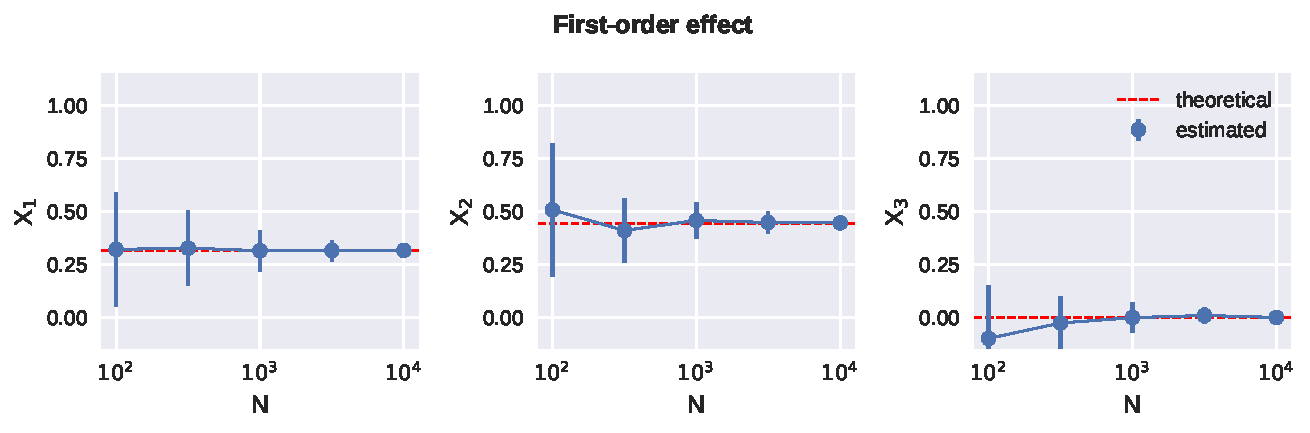
\includegraphics[width=\linewidth]{figures/chapterA/Ishigami_S1.pdf}}\quad
    \subfloat[Total effects.]
    {\label{fig:ishigami_st_theo}
    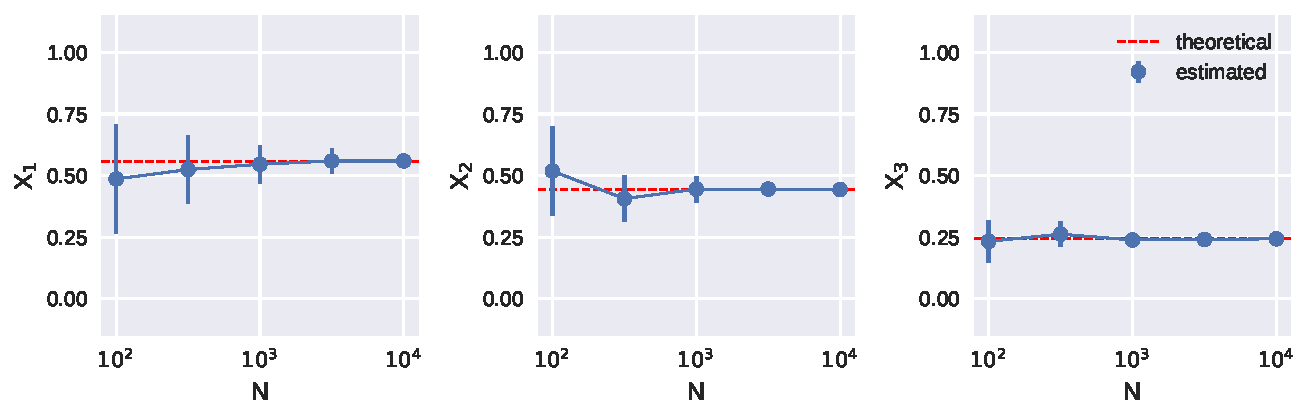
\includegraphics[width=\linewidth]{figures/chapterA/Ishigami_ST.pdf}}
    \caption{Ishigami function Sobol' first-order (main) and total sensitivity indices estimated using the simulator. Indices are given as pointwise estimates with bootstrap $\SI{95}{\percent}$ confidance intervals.}
    \label{fig:ishigami_simulator_estimates}
\end{figure}

\begin{table}[ht!]
    \myfloatalign
    \begin{tabularx}{\textwidth}{XXX}
    \toprule
    \tableheadline{Input factor} & \multicolumn{2}{c}{\spacedlowsmallcaps{Sobol' sensitivity index}} \\
    \midrule   
    & \tableheadline{$S_{i}$} & \tableheadline{$S_{Ti}$} \\
    \cmidrule{2-3}
    $X_{1}$   & $0.5607$ & $0.6705$ \\
    $X_{2}$   & $0.1402$ & $0.2063$ \\
    $X_{3}$   & $0.0623$ & $0.0958$ \\
    $X_{4}$   & $0.0350$ & $0.0547$ \\
    $X_{5}$   & $0.0224$ & $0.0353$ \\
    $X_{6}$   & $0.0156$ & $0.0246$ \\
    $X_{7}$   & $0.0114$ & $0.0181$ \\
    $X_{8}$   & $0.0088$ & $0.0139$ \\
    $X_{9}$   & $0.0069$ & $0.0110$ \\
    $X_{10}$  & $0.0056$ & $0.0089$ \\
    \bottomrule
    \end{tabularx}
    \caption{G*-function Sobol' first-order and total effects' theoretical values for $D=10$ and $\alpha_i=1$, $\delta_i\,\,\sim\,\,\mathcal{U}([0,\,1])$, $a_i=i-1$, for $i=1,\dots,D$.}
    \label{tab:gfun_theo_vals}
\end{table}

\begin{figure}[ht!]
    \myfloatalign
    \subfloat[Main effects.]
    {\label{fig:gstar_s1_theo}
    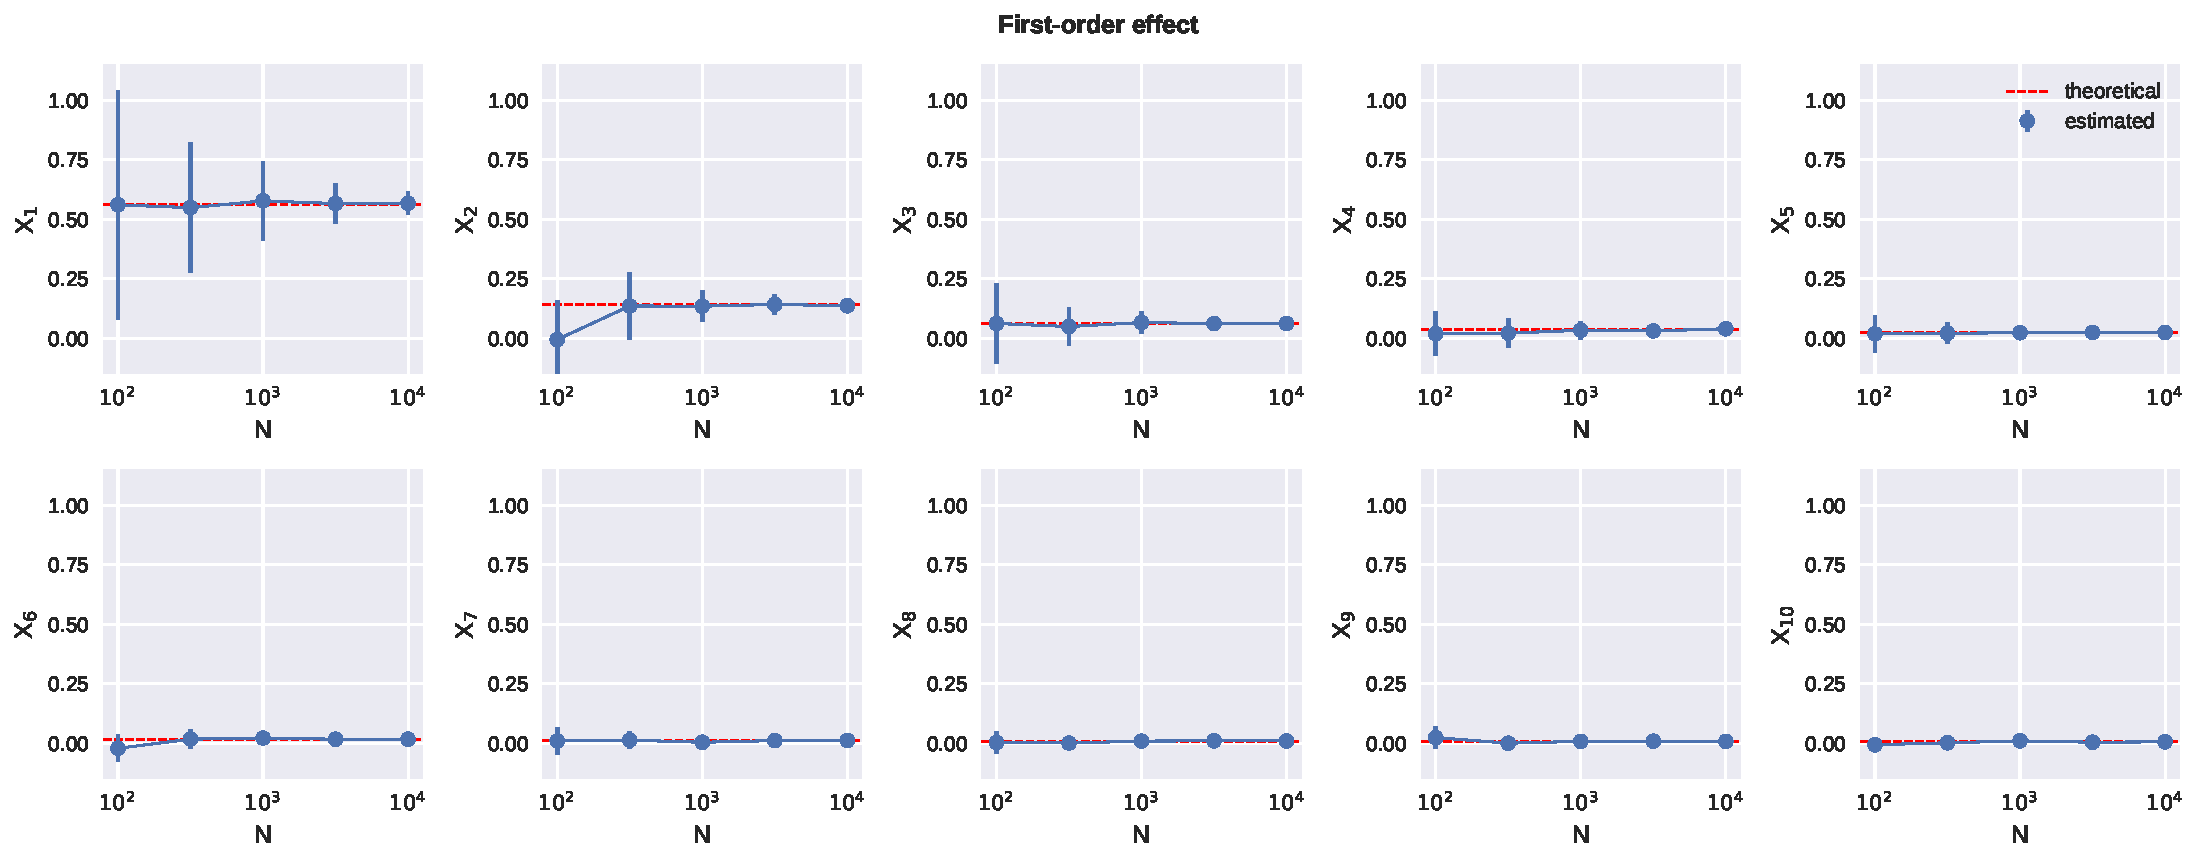
\includegraphics[width=\linewidth]{figures/chapterA/GStar_S1.pdf}}\quad
    \subfloat[Total effects.]
    {\label{fig:gstar_st_theo}
    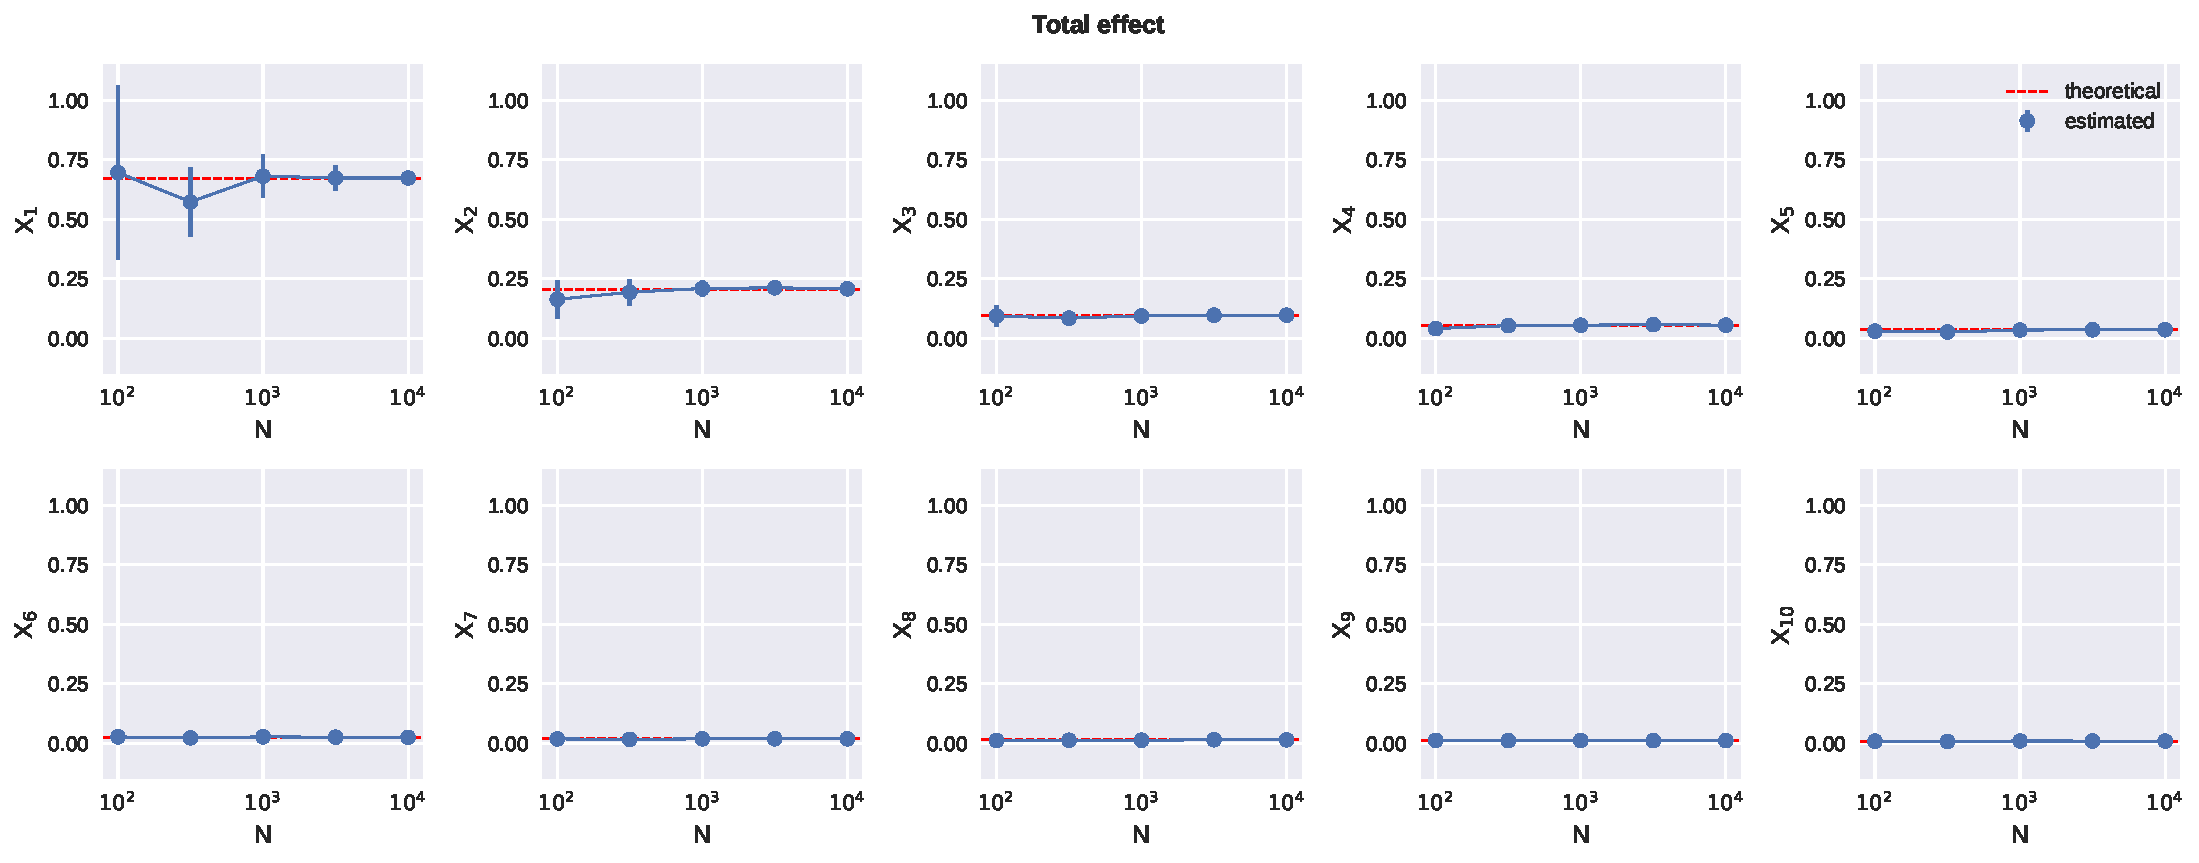
\includegraphics[width=\linewidth]{figures/chapterA/GStar_ST.pdf}}
    \caption{G*-function Sobol' first-order (main) and total sensitivity indices estimated using the simulator. Indices are given as pointwise estimates with bootstrap $\SI{95}{\percent}$ confidance intervals.}
    \label{fig:gstar_simulator_estimates}
\end{figure}


%
%
%
\clearpage
\subsection{Emulator estimates}\label{sec:chAemulator_estimates}
We wanted to test whether we could obtain reliable estimates of the Sobol' sensitivity indices this time by using emulators of the above presented test functions.

\vspace{0.2cm}
For this purpose, we sampled points $\mathbf{X}$ from a LHD over the hypercubes $[-\pi,\,\pi]^3$ and $[0,\,1]^{10}$ for the Ishigami and the G*- functions, respectively. We then simulated these points $Y=f_{simul}(\mathbf{X})$ to form a dataset $(\mathbf{X},\,Y)$ to be used as learning sample. The leaning sample size was given by $\vert\mathbf{X}\vert=\text{factor}\times D$, being $D$ the problem dimension ($D=3$ and $D=10$ for the Ishigami and G*- functions, respectively). Common practice for computer model experiments is to take at least $10\times D$ learning samples in Gaussian process regression settings~\cite{Rasmussen:2006}. In this study, we tested different multiplicative factors, taken from the set $\{10,\,20,\,30,\dots,\,100\}$. We also simulated an additional set of points (size $=\SI{20}{\percent}$ of the biggest learning sample used) to be used as a testing dataset for evaluating each of the trained emulators predictivity, as described by the coefficient of determination ($R^2$ score). After training and for each emulator, $1,000$ emulator posterior distribution's samples were used to obtain Sobol' sensitivity indices' distributions as described in Section~\ref{sec:ch3emulatorbasedestimates}. In this case, we only investigated the uncertainty in the estimates arising from the use of the emulators, while the quadrature formulae numerical errors were neglected (and not estimated using the bootstrap technique as done in Section~\ref{sec:chAsimulator_estimates}).

\vspace{0.2cm}
The obtained $R^2$ scores are summarised in Tables~\ref{tab:ifun_scores}--\ref{tab:gfun_scores} for the Ishigami and G*- functions, respectively. We can see that the emulator predictivity generally increases as the number of learning samples increases, although this behaviour eventually saturates, meaning that ``the more points'' does not always imply ``the better accuracy''. In Figures~\ref{fig:ishigami_emulator_estimates}--\ref{fig:gstar_emulator_estimates}, the estimated Sobol' sensitivity indices are compared with the respective theoretical values. The estimated values are given as distributions, and each distribution is plotted against the multiplicative factor used to build the training dataset of the corresponding emulator which was used to obtain the distribution itself. We can see that the distributions progressively center around (i.e. their mean values match) the theoretical values as the number of learning samples used to train the emulator increases. In particular, for both the Ishigami and G*- functions we can see that at least $40\times D$ learning samples were necessary to achieve a satisfactory match with theoretical values. Again, we cannot derive absolute statements concerning what is the optimal choice of the multiplicative factor, and investigating this goes beyond the scope of the project. Nevertheless, we have demonstrated the feasibility of estimating Sobol' sensitivity indices with good accuracy by using emulators of both example $3$D and $10$D nonlinear and nonmonotonic computer codes.

\newpage
\begin{table}[ht!]
    \myfloatalign
    \begin{tabularx}{0.5\textwidth}{XX}
    \toprule
    \tableheadline{Factor} & \tableheadline{$R^2$ score} \\
    \midrule
    $10\times$   & $0.3796$ \\
    $20\times$   & $0.5187$ \\
    $30\times$   & $0.5438$ \\
    $40\times$   & $0.8563$ \\
    $50\times$   & $0.9526$ \\
    $60\times$   & $0.9770$ \\
    $70\times$   & $0.9806$ \\
    $80\times$   & $0.9862$ \\
    $90\times$   & $0.9876$ \\
    $100\times$  & $0.9941$ \\
    \bottomrule
    \end{tabularx}
    \caption{Ishigami function emulators' predictivity as described by the $R^2$ score. Predictivity is tested against the same set of points for each of emulators trained on differently large training datasets.}
    \label{tab:ifun_scores}
\end{table}

\begin{figure}[ht!]
    \myfloatalign
    \subfloat[Main effects.]
    {\label{fig:ishigami_s1_theo}
    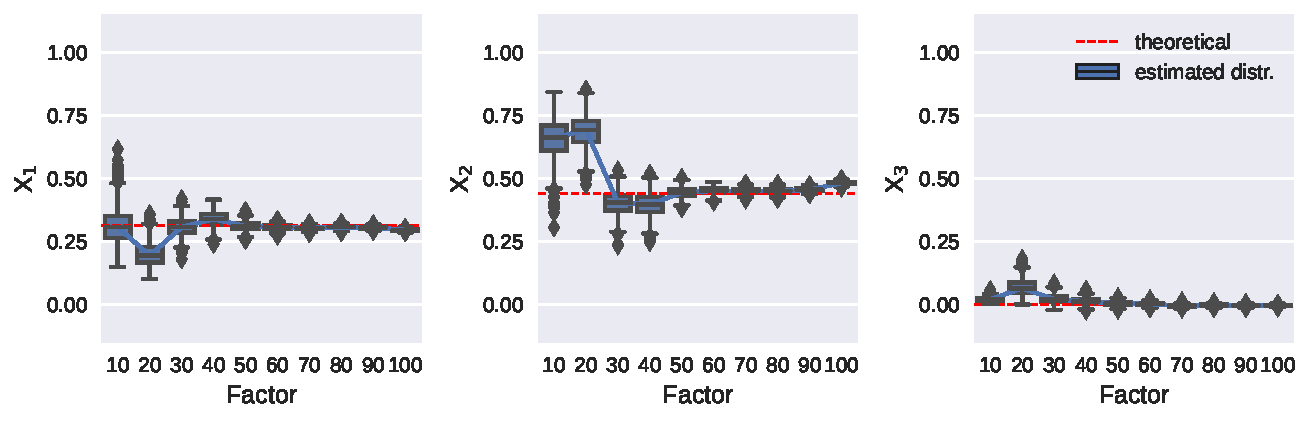
\includegraphics[width=\linewidth]{figures/chapterA/Ishigami_S1_gpe_based.pdf}}\quad
    \subfloat[Total effects.]
    {\label{fig:ishigami_st_theo}
    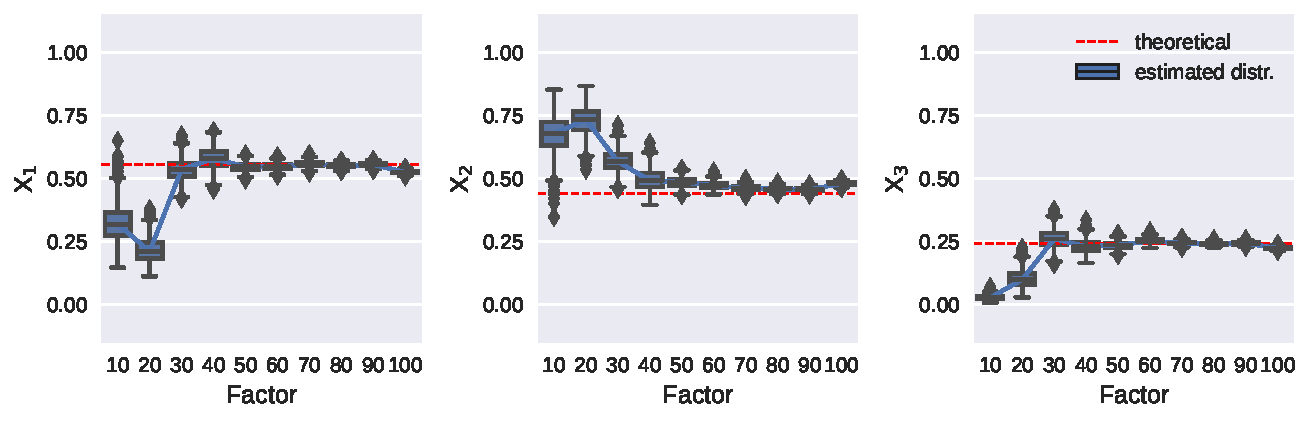
\includegraphics[width=\linewidth]{figures/chapterA/Ishigami_ST_gpe_based.pdf}}
    \caption{Ishigami function Sobol' first-order (main) and total sensitivity indices estimated using the emulator. Indices are given as different estimates (forming entire distributions) corresponding to different samples from the full emulators' posterior distributions.}
    \label{fig:ishigami_emulator_estimates}
\end{figure}

\begin{table}[ht!]
    \myfloatalign
    \begin{tabularx}{0.5\textwidth}{XX}
    \toprule
    \tableheadline{Factor} & \tableheadline{$R^2$ score} \\
    \midrule
    $10\times$   & $0.6470$ \\
    $20\times$   & $0.7689$ \\
    $30\times$   & $0.7534$ \\
    $40\times$   & $0.7881$ \\
    $50\times$   & $0.8332$ \\
    $60\times$   & $0.8396$ \\
    $70\times$   & $0.8427$ \\
    $80\times$   & $0.8569$ \\
    $90\times$   & $0.8805$ \\
    $100\times$  & $0.8896$ \\
    \bottomrule
    \end{tabularx}
    \caption{G*-function emulators' predictivity as described by the $R^2$ score. Predictivity is tested against the same set of points for each of emulators trained on differently large training datasets.}
    \label{tab:gfun_scores}
\end{table}

\begin{figure}[ht!]
    \myfloatalign
    \subfloat[Main effects.]
    {\label{fig:gstar_s1_theo}
    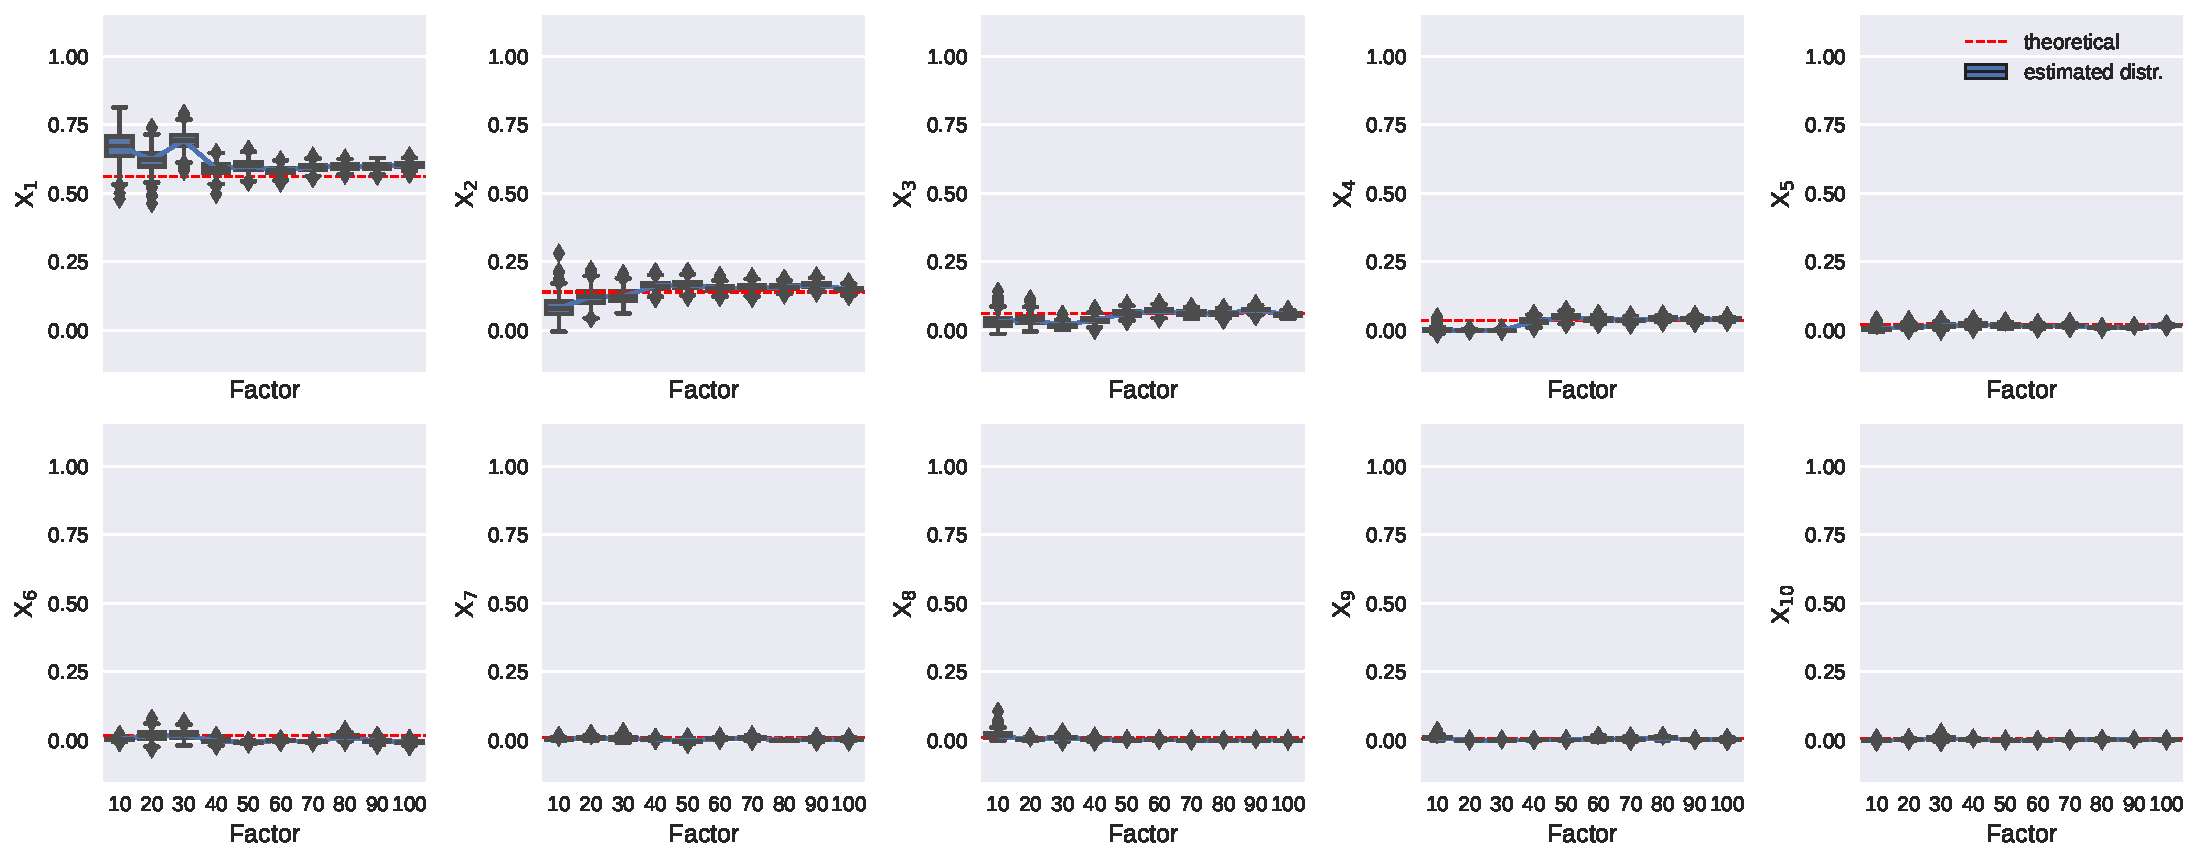
\includegraphics[width=\linewidth]{figures/chapterA/GStar_S1_gpe_based.pdf}}\quad
    \subfloat[Total effects.]
    {\label{fig:gstar_st_theo}
    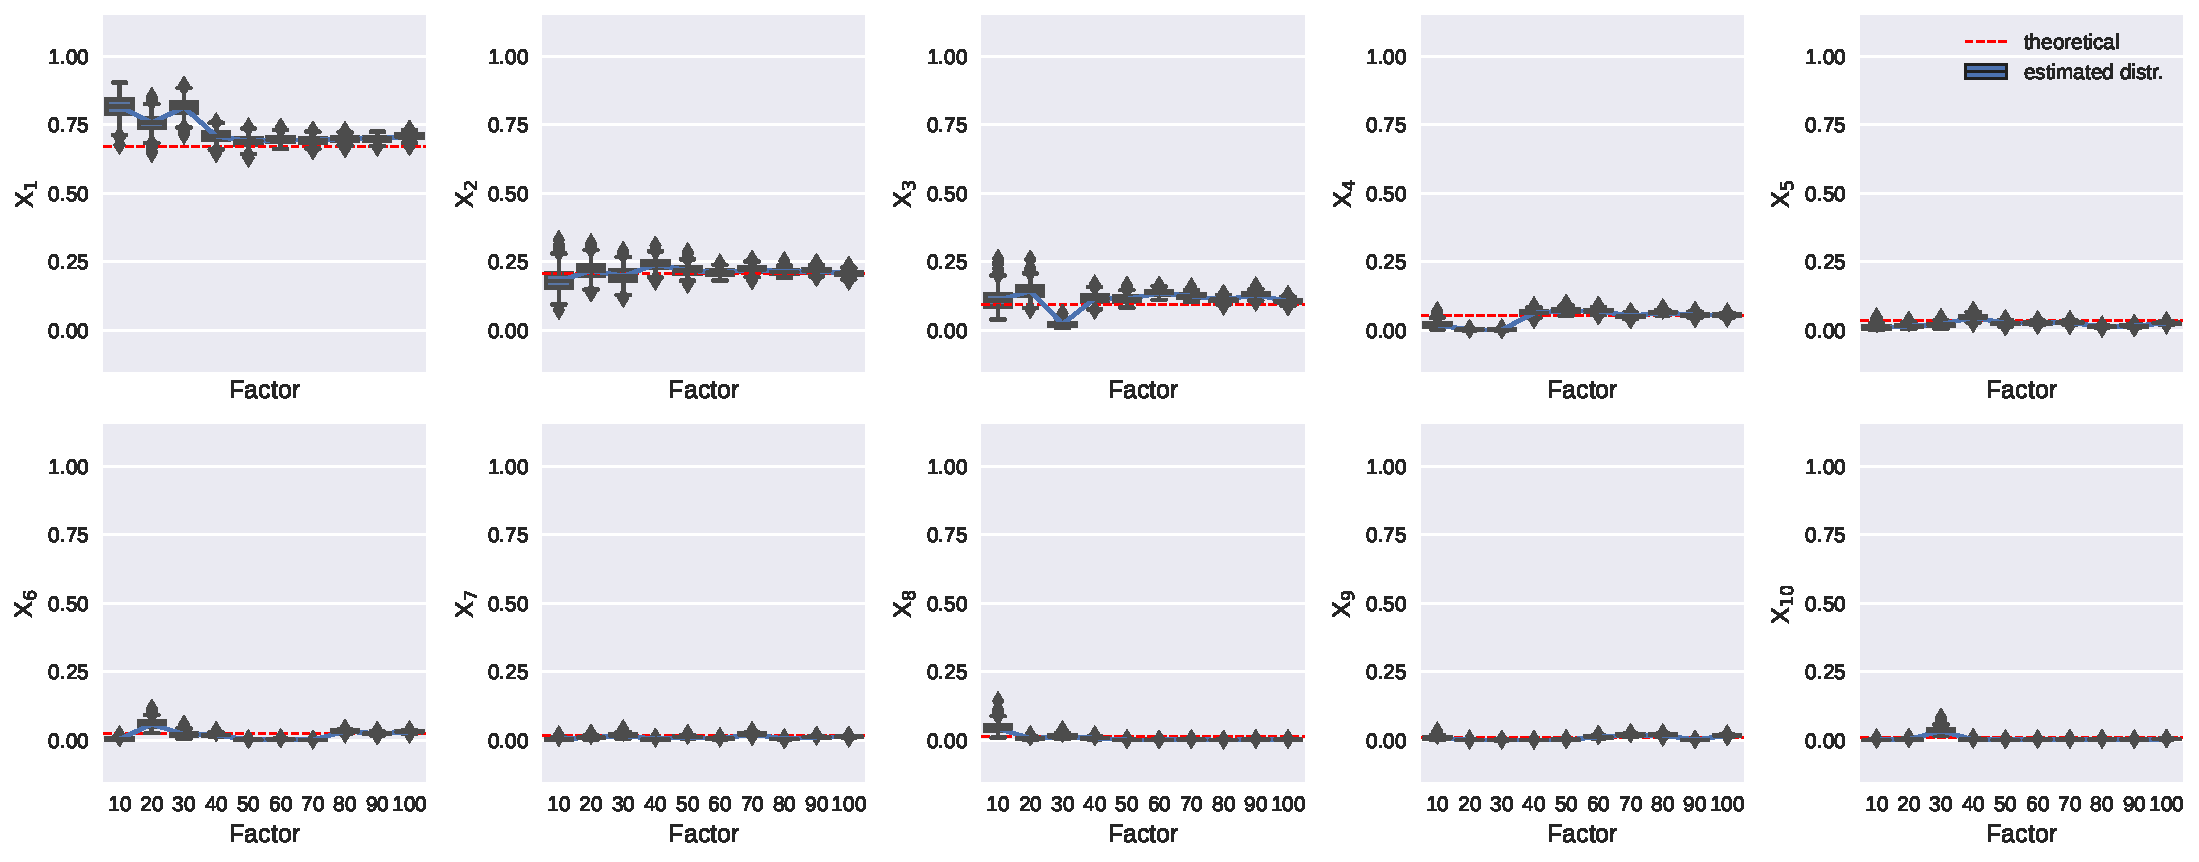
\includegraphics[width=\linewidth]{figures/chapterA/GStar_ST_gpe_based.pdf}}
    \caption{G*-function Sobol' first-order (main) and total sensitivity indices estimated using the emulator. Indices are given as different estimates (forming entire distributions) corresponding to different samples from the full emulators' posterior distributions.}
    \label{fig:gstar_emulator_estimates}
\end{figure}


%
%
%
\cleardoublepage
\section{HM validation using synthetic data}\label{sec:chAHM_validation_using_synthetic_data}
We validated HM technique against \textit{synthetic data}, generated using the \textit{in silico} model of SHAM rat heart contraction mechanics (Section~\ref{sec:ch4ratheartcontractionmodel}).

\vspace{0.2cm}
For this purpose, we started from the performed HM on the SHAM model (Section~\ref{sec:ch4modelfitting}, Figure~\ref{fig:shamhm}). We selected an intermediate wave, specifically wave $4$, among the total $8$ waves the full process took to complete (Figure~\ref{fig:hm1}). We then sampled $256$ points in wave $4$ that did not belong to the final wave, namely wave $8$ (Figures~\ref{fig:hm2}--\ref{fig:hm3}). We then simulated all these points and computed the LV features' mean and standard deviation values for the ones that led to a converging simulation ($48$ points). We further used these mean and standard deviation values as synthetic data to be matched. The LV features' synthetic variability is summarised in Table~\ref{tab:values2match4synt}.

\begin{table}[ht!]
    \myfloatalign
    \begin{tabularx}{\textwidth}{lXX}
    \toprule
    \tableheadline{LV feature} & \tableheadline{Units}                  & \tableheadline{Synthetic variability} \\
    \midrule
    $\textrm{EDV}^{*}$         & $\SI{}{\micro\liter}$                  & $493.10 \pm 16.85$ \\
    $\textrm{ESV}^{*}$         & $\SI{}{\micro\liter}$                  & $204.29 \pm  7.93$ \\
    $\textrm{EF}$              & $\SI{}{\percent}$                      & $ 58.54 \pm  1.74$ \\
    $\textrm{IVCT}$            & $\SI{}{\milli\second}$                 & $140.86 \pm  0.78$ \\
    $\textrm{ET}^{*}$          & $\SI{}{\milli\second}$                 & $ 56.77 \pm  1.53$ \\
    $\textrm{IVRT}^{*}$        & $\SI{}{\milli\second}$                 & $ 20.03 \pm  2.43$ \\
    $\textrm{Tdiast}$          & $\SI{}{\milli\second}$                 & $ 94.07 \pm  1.11$ \\
    $\textrm{PeakP}^{*}$       & $\SI{}{\kilo\pascal}$                  & $ 18.56 \pm  1.14$ \\
    $\textrm{Tpeak}$           & $\SI{}{\milli\second}$                 & $ 39.39 \pm  1.36$ \\ 
    $\textrm{ESP}$             & $\SI{}{\kilo\pascal}$                  & $ 8.74  \pm  0.21$ \\
    $\textrm{maxdP}^{*}$       & $\SI{}{\kilo\pascal\per\milli\second}$ & $ 1.08  \pm  0.06$ \\
    $\textrm{mindP}^{*}$       & $\SI{}{\kilo\pascal\per\milli\second}$ & $-0.54  \pm  0.06$ \\
    \bottomrule
    \end{tabularx}
    \caption{Synthetic data LV features' variability given as mean $\pm$ standard deviation values to match for HM validation. Only the LV features with an asterisk $(\,\,)^*$ were used as targets for HM.}
    \label{tab:values2match4synt}
\end{table}

\vspace{0.2cm}
We started the HM process from the same initial space-filling design (lightest blue variant coloured points in Figure~\ref{fig:shamhm}) used for the SHAM model HM, this time trying to match the synthetic data instead of the experimental data. To replicate exactly the same process, we tried to match the same $7$ features out of the total $12$ features of interest, although we had mean and standard deviation values for all the LV features. Figure~\ref{fig:syntfeatmatch} shows that all the LV features were perfectly matched at the end of the HM process (which took $9$ waves to complete), including the $5$ features we did not directly selected as targets for HM.

\begin{figure}[ht!]
    \myfloatalign
    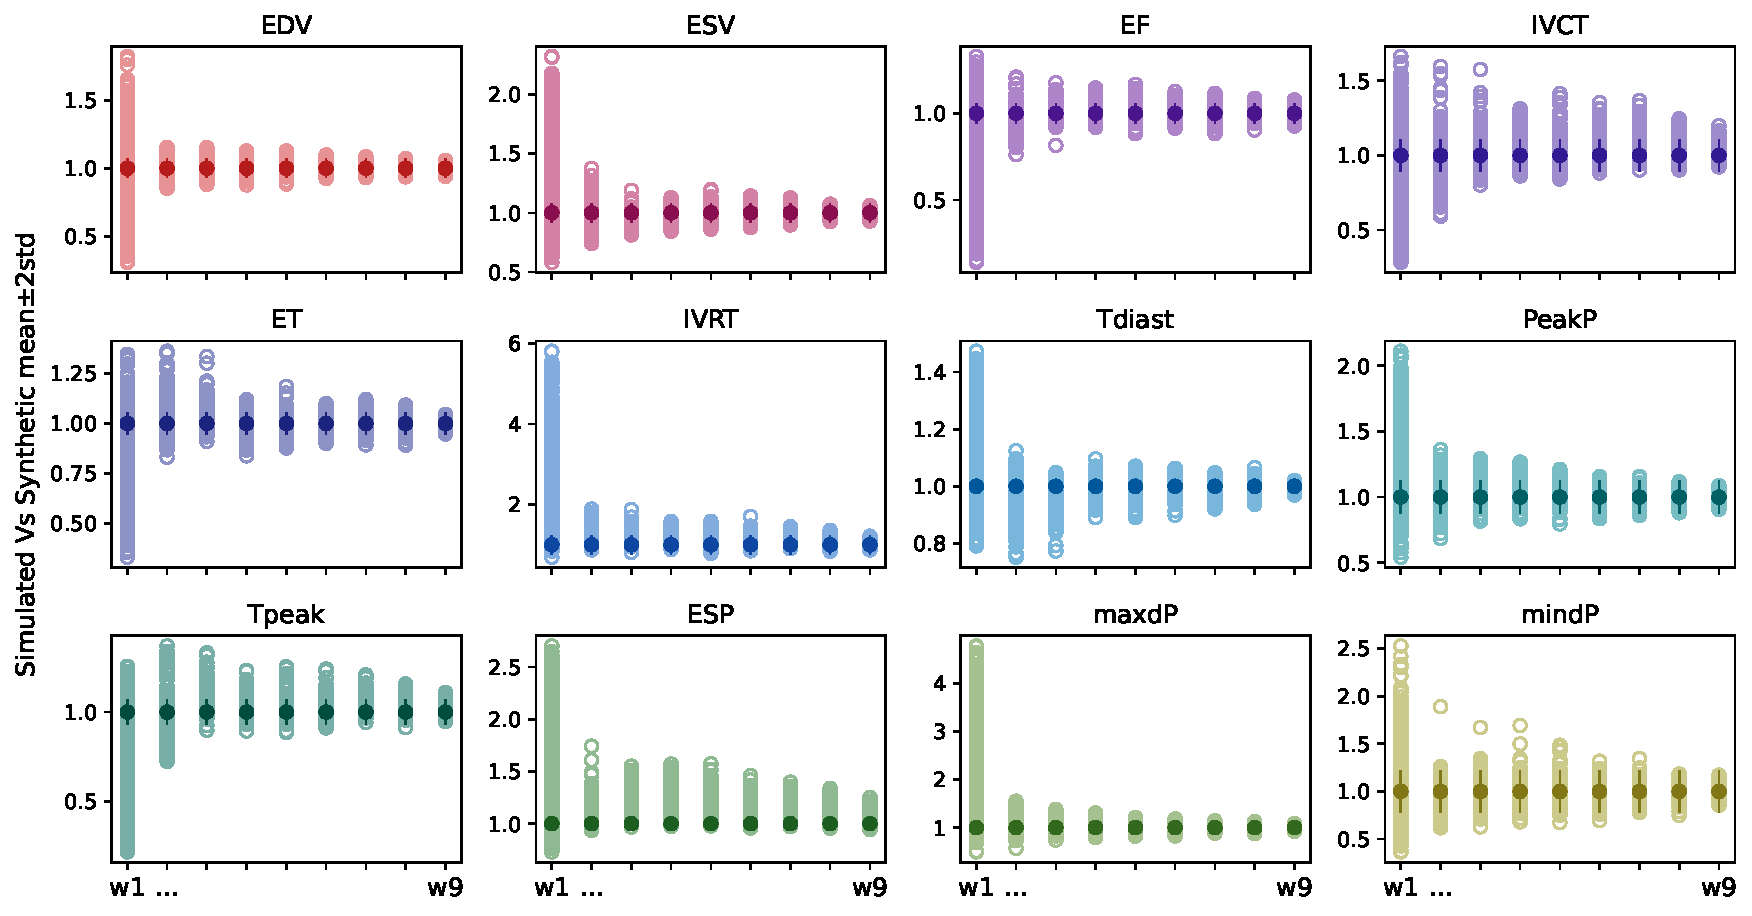
\includegraphics[width=1\textwidth]{figures/chapterA/hm_vs_synt_data_features.pdf}
    \caption{Simulated LV features’ distributions around synthetic mean values. These are obtained by evaluating the simulator at input parameter points belonging to the first (w$1$) up to the last (w$9$) waves of HM performed on synthetic data. Simulated features are shown as empty dots, while the related synthetic mean values are displayed as full dots. $2$ STD confidence intervals are also shown as vertical straight lines centred around synthetic mean values. All the displayed values (including confidence intervals) are normalised by their respective synthetic mean values.}
    \label{fig:syntfeatmatch}
\end{figure}

\vspace{0.2cm}\noindent
Moreover, we can see that the input parameters' ranges characterising the non-implausible $X_{NIMP}$ space of the last HM wave were most of the time restricted to ranges which have non-empty intersection with the ranges where the synthetic data were sampled from (Figure~\ref{fig:syntintmatch}). This shows that HM technique not only matched the target features' values but also recovered the initial sample space.

\begin{figure}[ht!]
    \myfloatalign
    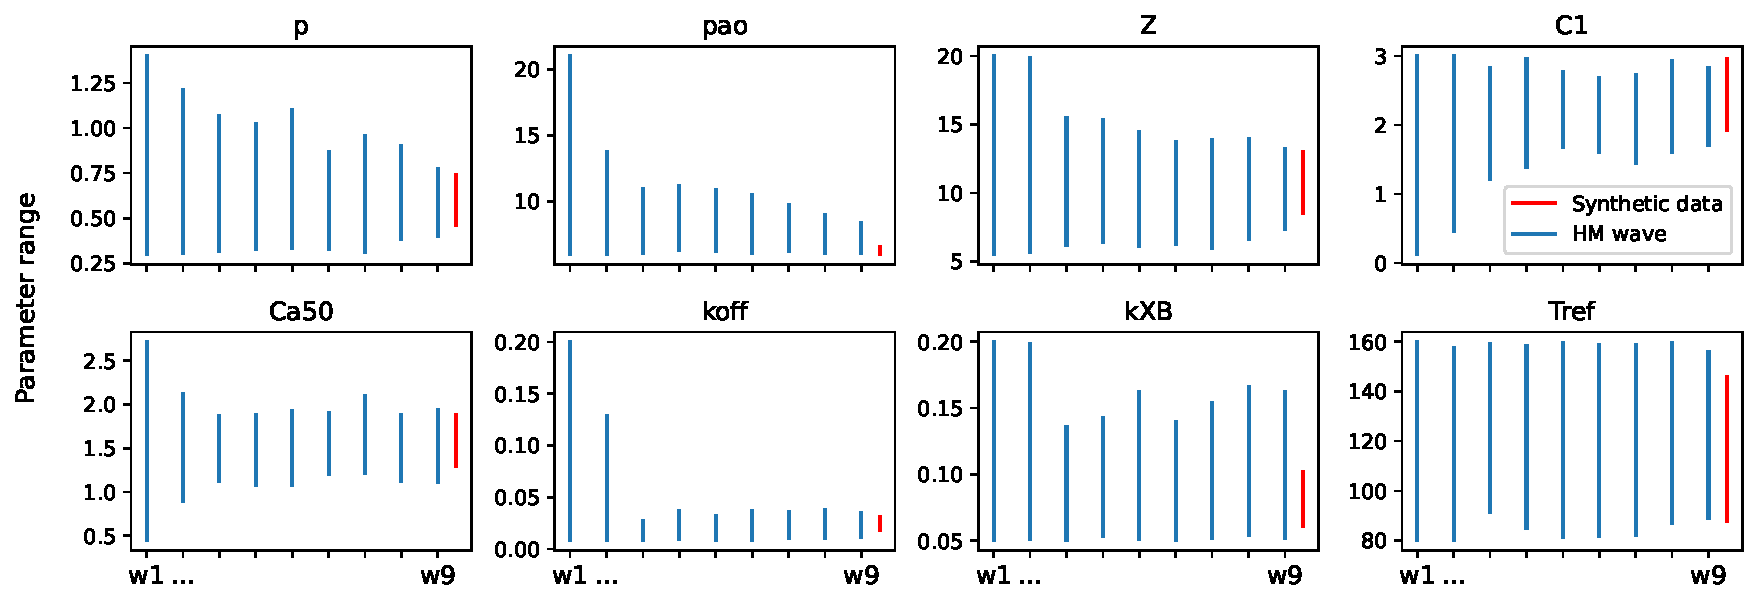
\includegraphics[width=1\textwidth]{figures/chapterA/hm_vs_synt_data_parameters.pdf}
    \caption{Input parameters' ranges at each wave during SHAM rat heart model HM on synthetic data (blue). The parameters' ranges where the synthetic data were sampled from are also shown (red).}
    \label{fig:syntintmatch}
\end{figure}

\begin{figure}[ht!]
    \myfloatalign
    \subfloat[The initial space with wave $4$ and wave $8$ $X_{NIMP}$ spaces is highlighted.]
    {\label{fig:hm1}
    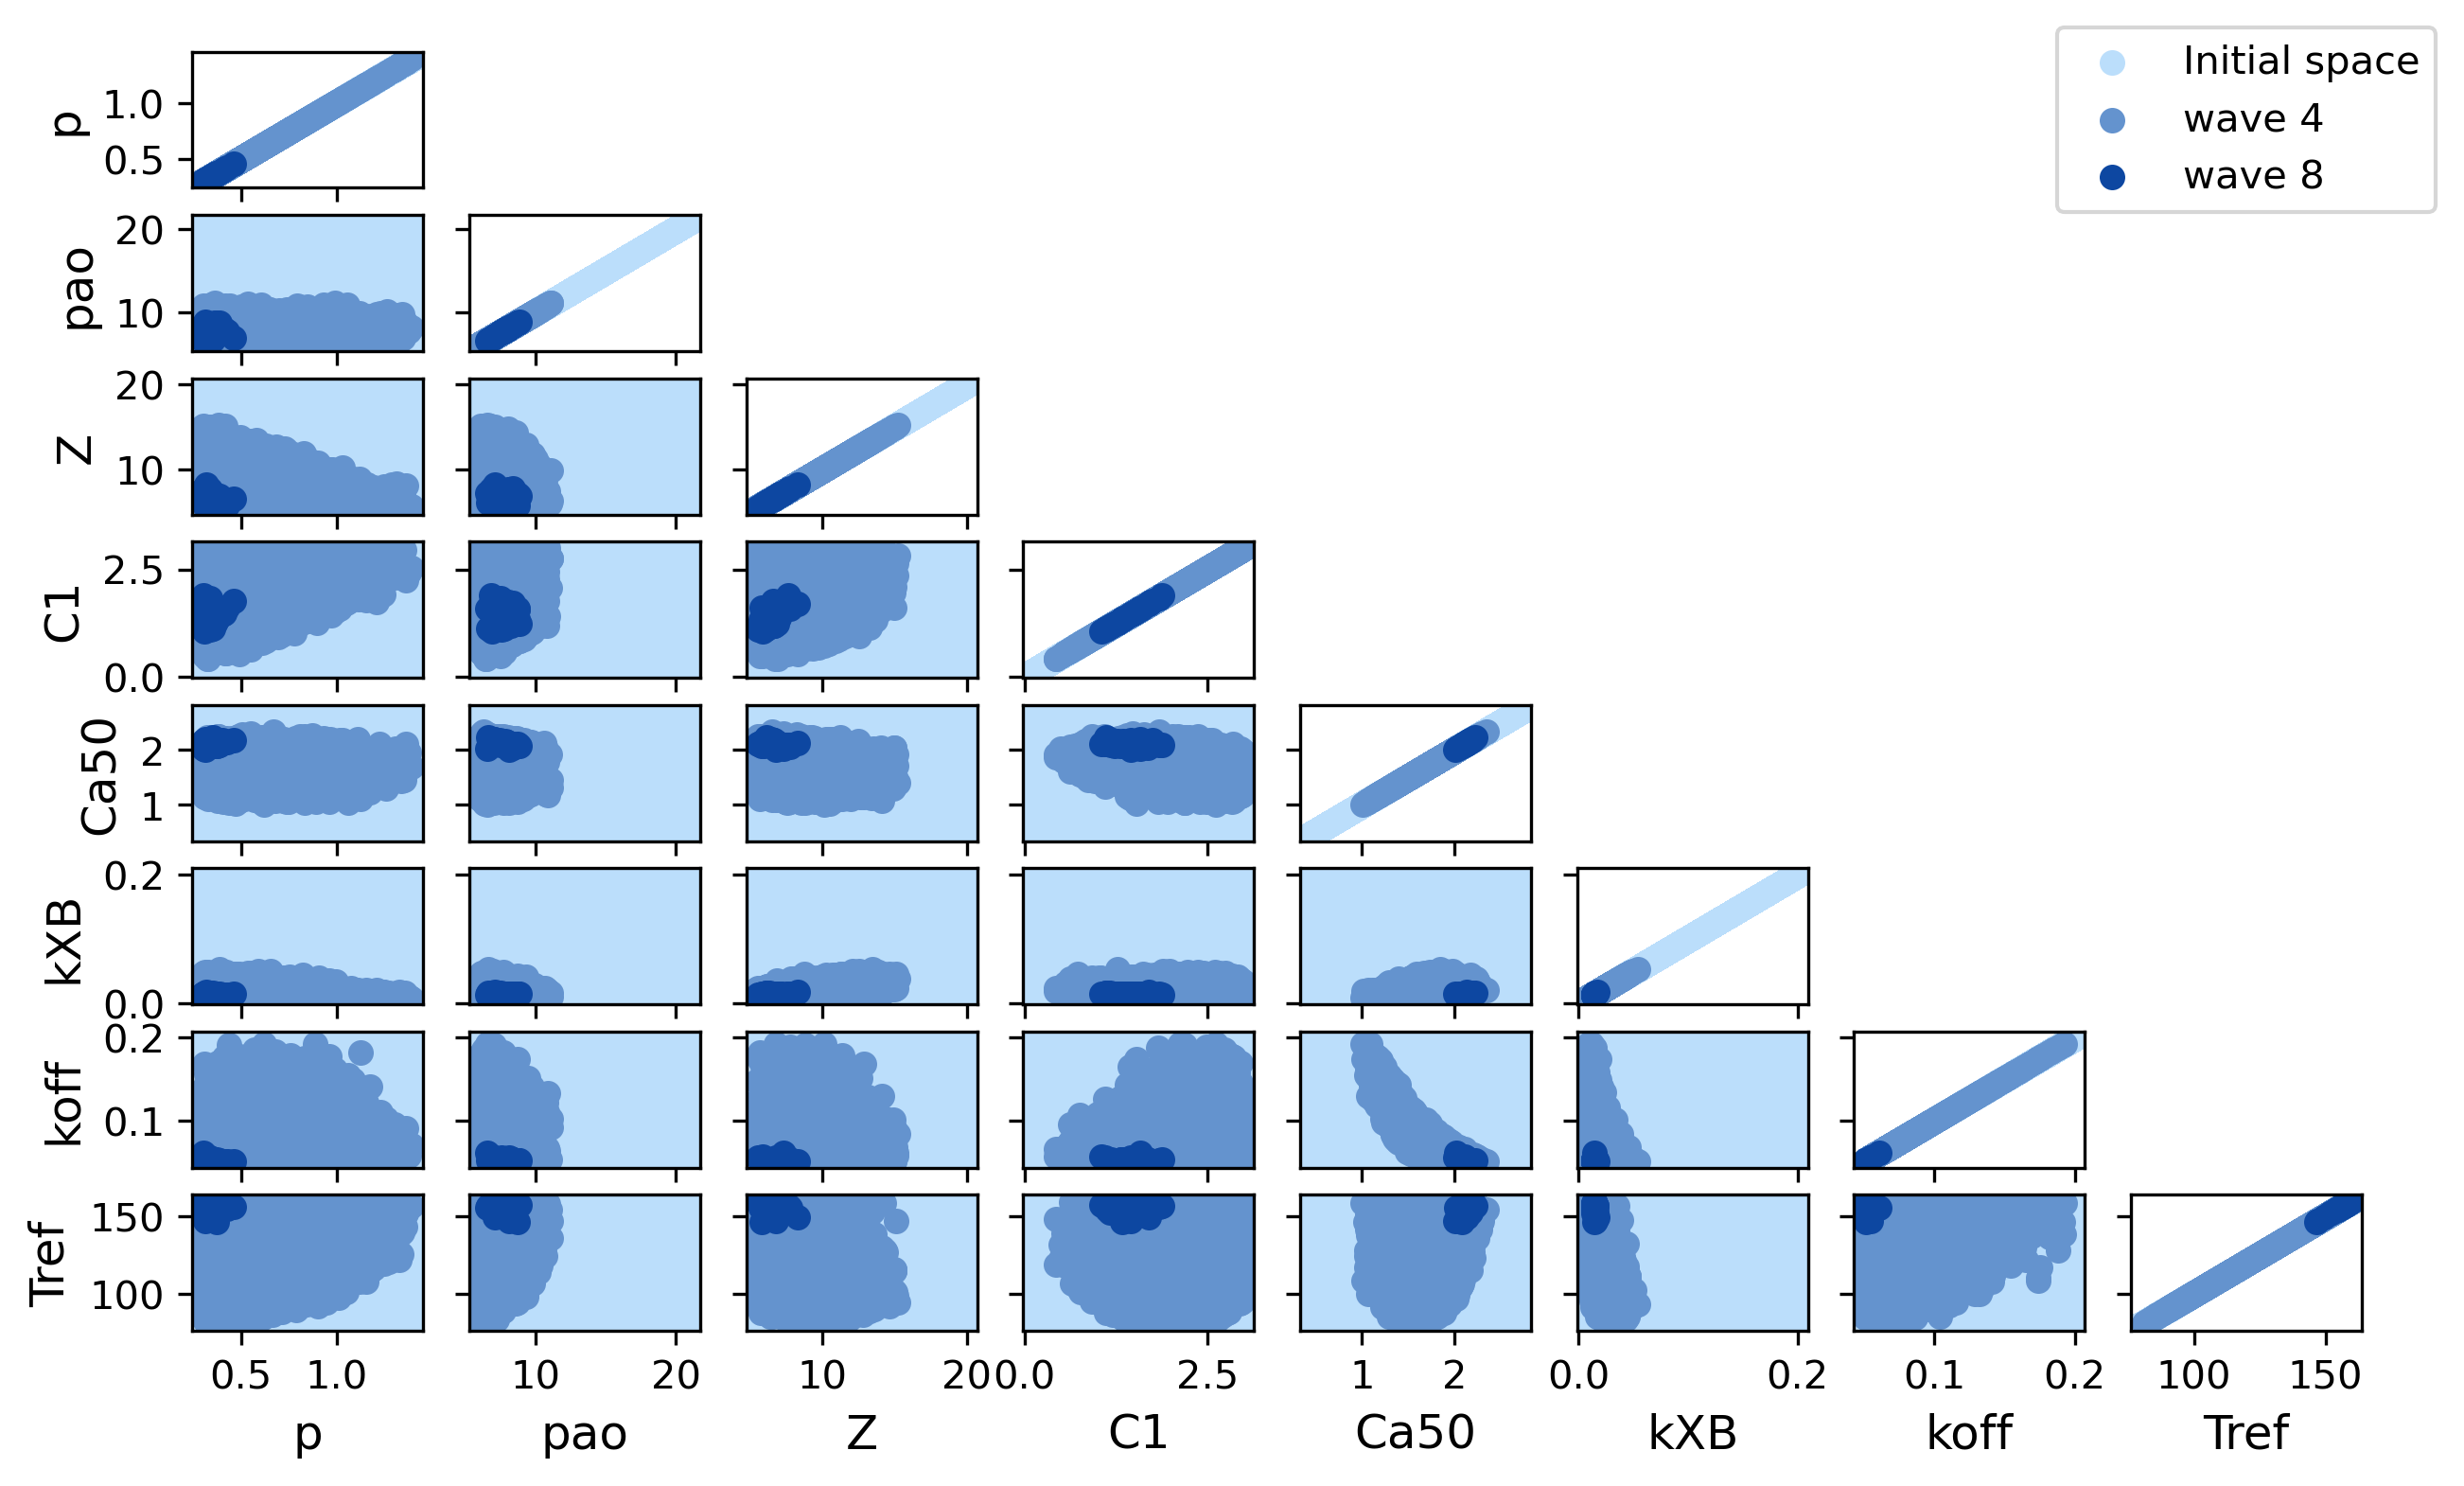
\includegraphics[width=\linewidth]{figures/chapterA/1_initial_w4_w8.png}}\quad
    \subfloat[Wave $8$ $X_{NIMP}$ space is cut out of the full space.]
    {\label{fig:hm2}
    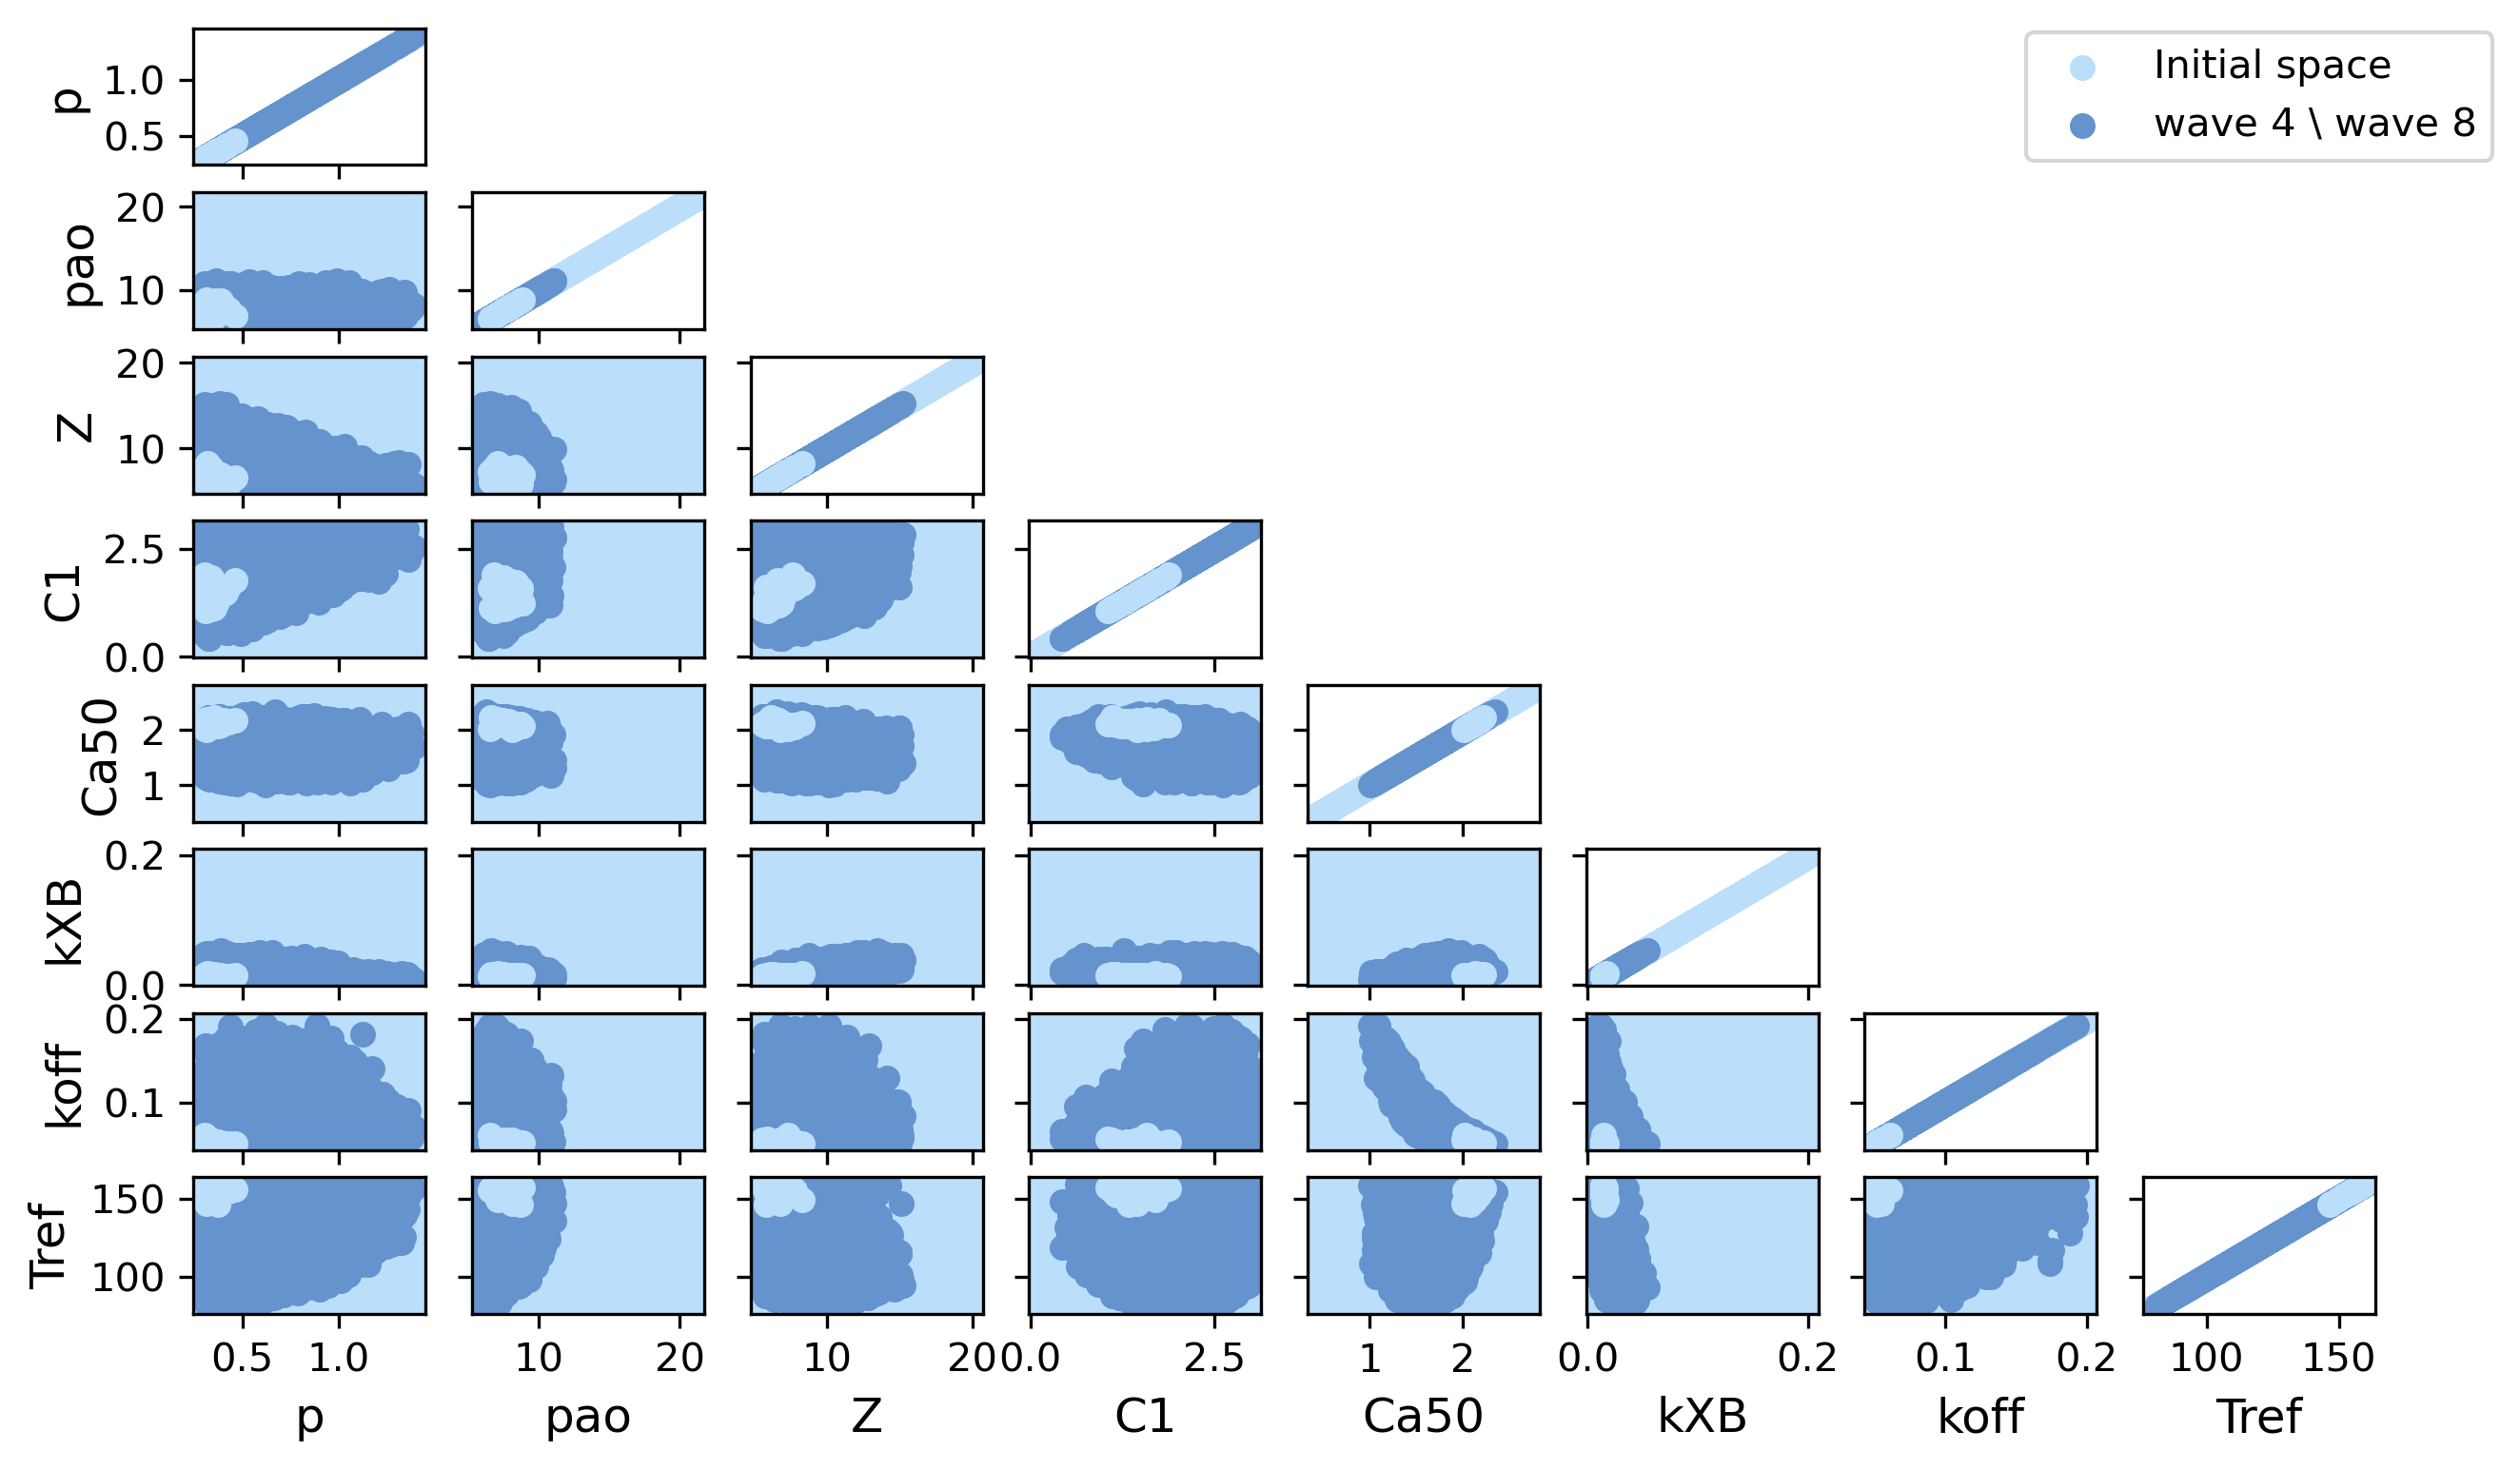
\includegraphics[width=\linewidth]{figures/chapterA/2_initial_w4minusw8.png}}\quad
    \subfloat[Points are sampled within wave $4$ $X_{NIMP}$ but not within wave $8$ $X_{NIMP}$ space.]
    {\label{fig:hm3}
    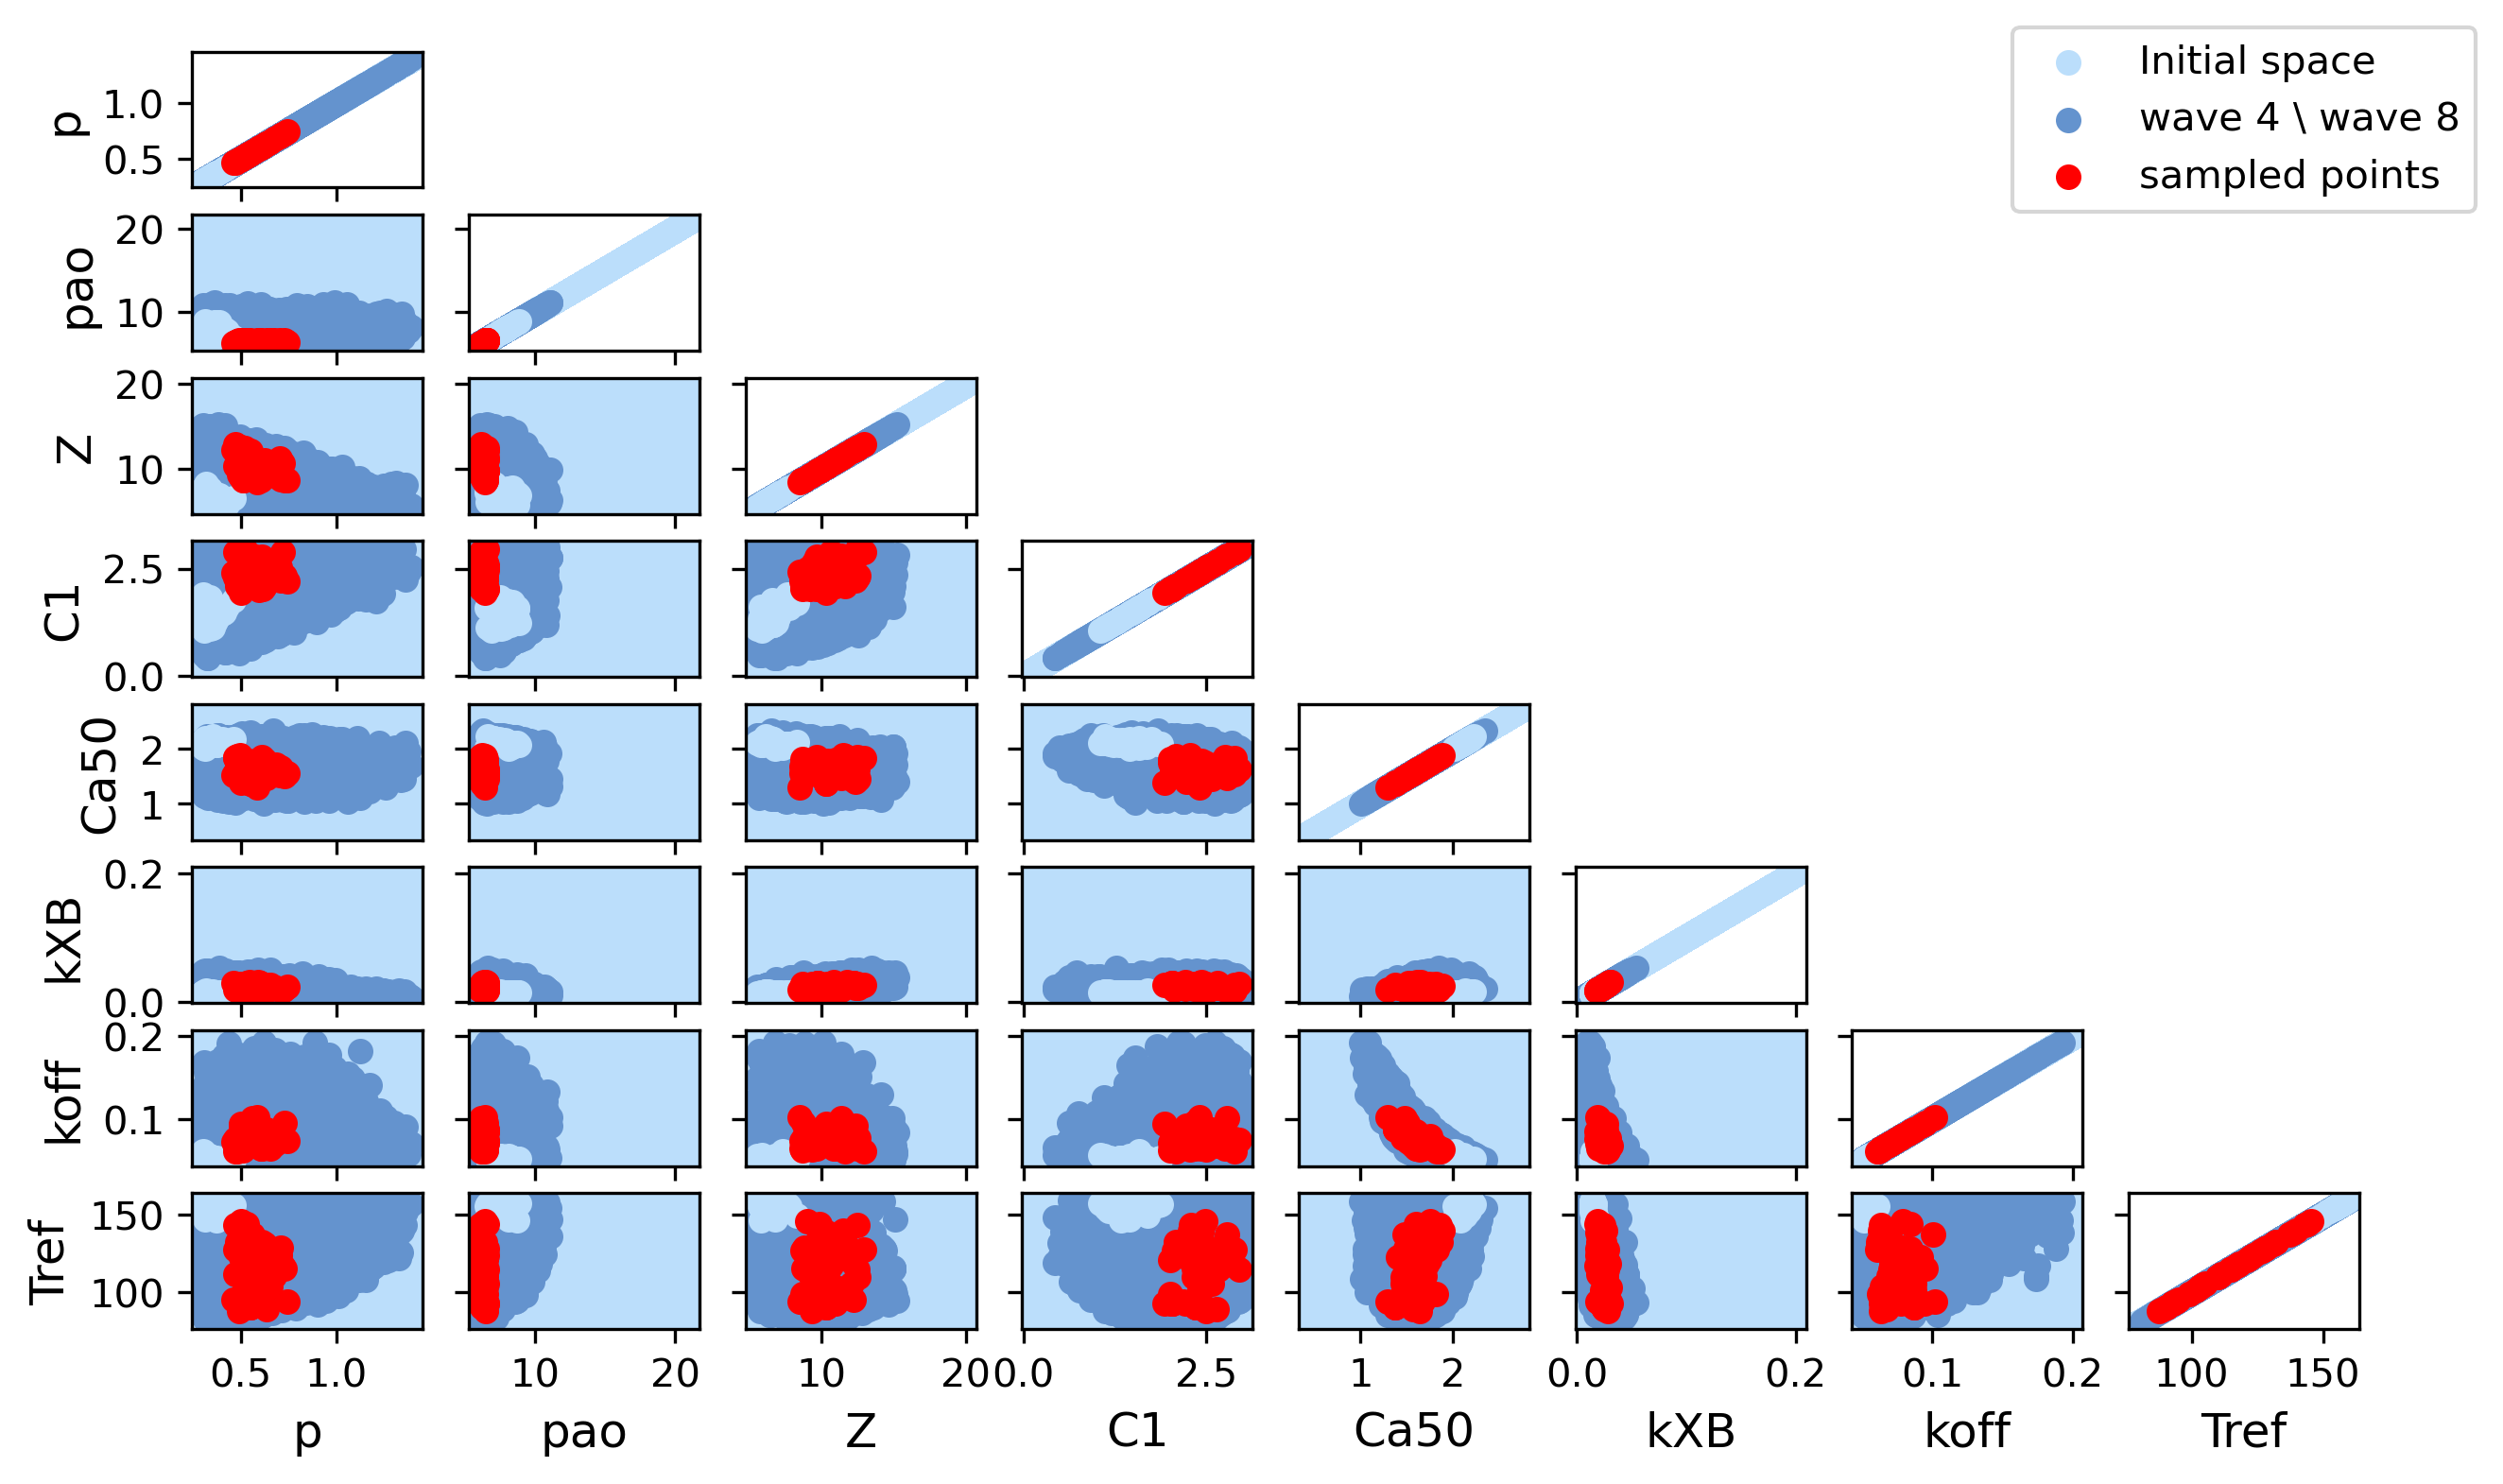
\includegraphics[width=\linewidth]{figures/chapterA/3_initial_w4minusw8_sampledpoints.png}}
    \caption{The process of points' selection for synthetic data generation to be used for HM technique validation.}\label{fig:ratrepimag}
\end{figure}